%\chapter{det-comp}

%%%%%%%%%%%%%%%%%%%%%%%%%%%%%%%%%%%%%%%%%%%%%%
\section{Anode Plane Assemblies (APA)}

%%%%%%%%%%%%%%%%%%%%%%%%%%
\subsection{Scope and requirements}

Anode Plane Assemblies (APAs) are the detector elements utilized to sense ionization created by charged particles traversing the liquid argon volume inside the single-phase TPC.  
An APA is constructed from a framework of lightweight, rectangular stainless steel tubing, with
four layers of wires wrapped on each side of the frame; the wrapping is illustrated in  Figure~\ref{fig:tpc_apa1}. From the outside in, the first wire layer
is a shielding (grid) plane, next are two induction planes and the collection plane. The front-end
electronics boards are mounted on one end of the APA frame and protected by a metal enclosure.
The APAs are 2.3 m wide, 6.3 m high, and 12 cm thick. The height is chosen for fabrication
purposes and compatibility with underground transport limitations. The 2.3-m width is set to fit
in a standard High Cube container for storage and transport with sufficient shock absorbers and
clearances.
ProtoDUNE-SP will feature six APAs, arranged in two rows of three, flanking either side of a central cathode plane.  

\begin{cdrfigure}[APA Diagram]{tpc_apa1}{Sketch of a ProtoDUNE-SP APA. This shows only portions of each of the three wire layers, U (green), V (magenta) and X (blue), to accentuate their angular relationships to the frame and to each other.  All layers span the entire APA frame height. The induction layers (U and V) are connected electrically across both sides of the APA.  The wires in the grid layer, G (not shown), run vertically, parallel to the X layer wires.  A mesh layer is attached directly to the APA frame.}
\includegraphics[width=0.8\textwidth, angle=90]{figures/tpc_apa1.png} 
\end{cdrfigure}


The initial physics performance requirements that drive the design of the APA are listed in Table \ref{tab:physicsrequirements}.  These are chosen to enable ProtoDUNE-SP to perform high-efficiency reconstruction throughout the entire active volume of the LArTPC, across the broad range of particle momenta and species present in the beam.  

\begin{cdrtable}[APA Physics Requirements]{lr}{physicsrequirements}{Preliminary physics requirements that motivate APA design parameters.}   
Requirement & Value  \\ \toprowrule
MIP Identification & 100$\%$ efficiency \\ \colhline
High efficiency for charge reconstruction & $>$90$\%$ for $>$100 MeV \\ \colhline
Vertex Resolution (x,y,z) & (1.5 cm, 1.5 cm, 1.5 cm)\\ \colhline
\textbf{Particle Identification} & \\ 
Muon Momentum Resolution & $<$18$\%$ for non-contained \\
            & $<$5$\%$ for contained\\ 
Muon Angular Resolution & $<$1$^{\circ}$\\            
Stopping Hadrons Energy Resolution & 1-5$\%$\\
Hadron Angular Resolution & $<$10$^{\circ}$ \\ \colhline
\textbf{Shower identification} & \\
Electron efficiency & $>$90$\%$\\
Photon mis-identification & $<$1$\%$\\
Electron Angular Resolution & $<$1$^{\circ}$ \\
Electron Energy Scale Uncertainty & $<$5$\%$\\
\end{cdrtable}

\fixme{The physics requirement table was added mostly for the APA review.  I would happily delete this and refer to some better table, if one is added to the Physics section. - MPS}

The ability to identify minimum-ionizing particles (MIPs) is a function of several detector parameters, including argon purity, drift distance, diffusion, wire pitch, and Equivalent Noise Charge (ENC).  ProtoDUNE-SP requires that MIPs originating anywhere inside the active volume of the detector be reconstructed with 100$\%$ efficiency.   The choice of wire pitch (i.e., $\sim$5 mm), combined with the design values of the other parameters just mentioned (and described in their respective sections of the TDR), should enable this 100$\%$ efficiency to be achieved for MIPs.


%\fixme{I had trouble getting the gist of this next pgraph; please see rewrite below it}
%Precisely identifying the location of any vertices in an event (e.g., the primary vertex in a neutrino interaction, or gamma conversion points in a $\pi^{0}$ decay) has direct impact on reconstruction efficiency.  The fine granularity of the LArTPC enables excellent performance in this task.  ProtoDUNE-SP requires a vertex resolution such that the fiducial volume, which among other factors determines the number of target nucleons that is a component in cross section measurements, in an analysis can be determined to $<$1$\%$.  This translates into a vertex resolution of $\sim$1.5 cm along each coordinate direction.  In practice, the resolution on the drift-coordinate ($x$) of a vertex/hit will be better than the resolution on its location in the $y-z$ plane, originating from the combination of drift-velocity and electronics sampling-rate.
%\fixme{double-check these vertex numbers, which are very likely incorrect at the moment.}

%\fixme{rewrite of above pgraph; if ok please delete previous paragraph} 
The fine granularity of the LArTPC enables excellent precision in identifying the location of any vertices in an event (e.g., the primary vertex in a neutrino interaction, or gamma conversion points in a $\pi^{0}$ decay), which has a direct impact on reconstruction efficiency. ProtoDUNE-SP requires that it be possible to determine the fiducial volume (via analysis) to $<$1$\%$, which requires reaching a vertex resolution of $\sim$1.5 cm along each coordinate direction. (The fiducial volume, among other factors, determines the number of target nucleons, which is a component in cross section measurements.) In practice, the resolution on the drift-coordinate ($x$) of a vertex or hit will be better than that on its location in the $y-z$ plane, due to the combination of drift-velocity and electronics sampling-rate.


%%%%%%%%%%%%
%\subsubsection{Overall physical description - connection to requirements.}
\subsection{APA design}
\label{subsec:apa_phys_desc}

%Figure \ref{fig:tpc_apa1} depicts a diagram of a ProtoDUNE-SP APA.  Each side of an APA consists of three layers of sense wires, plus additional grid and mesh layers.  Collection plane wires (labeled ``X'') span vertically from the bottom of the APA to the top.  There are two planes of induction wires (labeled ``U'' and ``V'') that wrap in a helical fashion, around the long edge of the APA, from the bottom of the APA to the top.  A grid layer (labeled ``G'') also spans from the bottom of the APA to the top, and is not connected for electronic readout.  The mesh layer (labeled ``M'') is secured directly to the APA frame, and effectively defines an equipotential plane over the entire surface area of the frame.  The arrangement of all layers, from the outside-in, is G-U-V-X-M. 
%
%\fixme{rewrite above pgraph}
Figure \ref{fig:tpc_apa1} depicts a ProtoDUNE-SP APA, each  side of which consists of three layers of sense wires, plus additional grid and mesh layers.  All wire layers span the entire height of the APA frame. Collection plane wires (labeled ``X'') run vertically.  Two planes of induction wires (labeled ``U'' and ``V'') wrap in a helical fashion around the long edge of the APA.  A grid layer (labeled ``G'') also spans the APA's height, but is not connected for electronic readout.  The mesh layer (labeled ``M'') is secured directly to the APA frame, and effectively defines an equipotential plane over the entire surface area of the frame.  The ordering of the layers, from the outside-in, is G-U-V-X-M. 

Table \ref{tab:apaparameters} lists some of the high-level parameters of the APA design.

% changed cc to lr
\begin{cdrtable}[APA Design Parameters]{lr}{apaparameters}{APA Design Parameters.}   
Parameter & Value  \\ \toprowrule
Active Height & 5.920 m\\ \colhline
Active Width & 2.295 m\\ \colhline
Wire Pitch (U,V) & 4.67 mm\\ \colhline
Wire Pitch (X,G) & 4.79 mm\\ \colhline
Wire Position Tolerance & 0.5 mm \\ \colhline
Wire Plane Spacing & 5 mm\\ \colhline
Wire Angle (w.r.t. vertical) (U,V) & 35.7$^{\circ}$\\ \colhline
Wire Angle (w.r.t. vertical) (X,G) & 0$^{\circ}$\\ \colhline
Number Wires / APA & 960 (X), 960 (G), 800 (U), 800 (V) \\ \colhline
Number Electronic Channels / APA & 2560 \\ \colhline
Wire Tension & 5.0 N \\ \colhline
Wire Material & Beryllium Copper \\ \colhline
Wire Diameter & 150 $\mu$m \\ \colhline
Wire Resistivity & 7.68 $\mu\Omega$-cm $@$ 20$^{\circ}$ C \\ \colhline
Wire Resistance/m & 4.4 $\Omega$/m $@$ 20$^{\circ}$ C \\ \colhline
Frame Planarity & 5 mm \\ \colhline
Photon Detector Slots & 10 \\
\end{cdrtable}


The operating voltages of the APA layers are listed in Table~\ref{tab:bias}.  When operated at these voltages, the drifting ionization follows trajectories around the grid and induction wires, ultimately terminating on a collection plane wire; i.e., the grid and induction layers are completely transparent to drifting ionization, and the collection plane is completely opaque.  The grid layer is present for pulse-shaping purposes, effectively shielding the first induction plane from the drifting charge and removing the long leading edge from the signals on that layer; again, it is not connected to the electronics readout. The mesh layer serves to shield the sense planes from pickup from the Photon Detection System and from ``ghost'' tracks that would otherwise be visible when ionizing particles have a trajectory that passes through the collection plane. 

\begin{cdrtable}[Baseline bias voltages for APA wire layers]{lr}{bias}{Baseline bias voltages for APA wire layers}   
Anode Plane & Bias Voltage  \\ \toprowrule
Grid (G) & -665 V\\ \colhline
Induction (U) & -370 V\\ \colhline
Induction (V) & 0 V\\ \colhline
Collection (X) & 820 V\\ \colhline
Mesh (M) & 0 V\\
\end{cdrtable}

The wrapped style allows the APAs to tile the active area of the LArTPC, minimizing the amount of dead space occupied by electronics and associated cabling.  The size of the APAs is chosen to be compatible with over-the-road shipping, and eventual transport to the 4850 level at SURF, into the membrane cryostat of a detector module.  The dimensions are also chosen such that an integral number of electronic readout channels and boards will fill in the full area of the APA. The modularity of the APAs allows them to be built and tested at off-site production facilities, decoupling their manufacturing time from the construction of the membrane cryostat.  

In the current design of the single-phase DUNE detector module, a central row of APAs is flanked by  drift-fields, requiring sensitivity on both sides. The wrapped APAs allow the induction plane wires to sense drifting ionization originating from either side of the APA.  This double-sided feature is not strictly necessary for the ProtoDUNE-SP arrangement, which has APAs located against the cryostat walls and a drift field on one side only, but it is compatible with this setup as the grid layer facing the wall effectively blocks any ionization outside the TPC from drifting in to the wires on that side of the APA.

Reconstruction of events recorded by the APAs will need to address ambiguities inherent to the wrapped wire design. This can occur when multiple isochronic hits are recorded, potentially leading to reconstructed hits that cannot be traced to unique wire-crossing positions in the detector.  The angle of the induction planes in the APA ($\pm$35.7$^{\circ}$) is chosen such that each induction wire only crosses a given collection wire one time, reducing the ambiguities that the reconstruction must address.  The design angle of the induction wires, coupled with their pitch, was also chosen such that an integer multiple of electronics boards reads out one APA.

The choices of wire tension and wire placement accuracy are made to ensure proper operation of the LArTPC at voltage, and to provide the precision necessary for reconstruction.  The tension of 5~N, when combined with the intermediate support combs that will be described in section \ref{subsec:apa_combs}, ensure that the wires are held taught in place with no sag.  Wire sag can impact the precision of reconstruction, as well as the transparency of the TPC.  The tension of 5~N is low enough that when the wires are cooled, which will increase their tension due to thermal contraction, they will stay safely below the break load of the beryllium copper wire, as described in section \ref{subsec:apa_wires}.  To further mitigate wire breakage and its impact on detector performance, each wire in the APA is anchored twice on both ends, with both solder and epoxy.  Details of this arrangement are provided in section \ref{subsubsec:apa_wire_wrap}. 


%%%%%%%%%%%%%%%%
%\subsection{APA Physical Description and Fabrication}
%%%%%%%%%%%%
\subsubsection{APA wires}
\label{subsec:apa_wires}

Beryllium copper (CuBe) wire is known for its high durability and yield strength. It is composed of $\sim$98$\%$ copper, approximately 1.9$\%$ beryllium, and a negligible amount of other elements. The DUNE APA wire has a diameter of 150$\mu$m (.006~in), and is strung in varying lengths across the apparatus. Three key properties for usage in the APA are: low resistivity, high tensile or yield strength, and coefficient of thermal expansion suitable for use with the APA's stainless steel frame.

Tensile strength of the wire describes the wire breaking stress (see Table \ref{tab:wire}).  The yield strength is the stress at which the wire starts to take a permanent (inelastic) deformation and is the important limit stress for our usage -- though most specifications give tensile strength.  Fortunately, for the CuBe alloys of interest, the two are fairly close to each other.  Based on the tensile strength of wire purchased from Little Falls Alloy (over 1380~MPa or 200,000~psi), the yield strength will be greater than 1100~MPa.  Given that the stress while in use is around 280~MPa, this leaves a comfortable margin.

The coefficient of thermal expansion (CTE) describes how material expands and contracts with changes in temperature.  The CTEs of CuBe alloy and 304 stainless steel are very similar.  Integrated down to 87~K, they are 2.7e-3 for stainless and 2.9e-3 for CuBe \fixme{find and add reference to bib file} (from study: ``Cryogenic Material Properties Database'' by Marquardt, Le and Radebaugh of NIST).

Since the wire contracts slightly more than the frame during cool-down the wire tension will go up.  If it starts at 5~N the tension will rise to about 5.5~N when everything is cool.  

The change in wire tension during cool-down could also be a concern.  In the worst case, the wire
 cools quickly to 87~K before any significant cooling of the frame  -- a realistic case because of the differing thicknesses.  In the limiting case, with complete contraction of the wire and none in the frame, the tension would be expected to reach $\sim$11.7 N.  This is still well under the $\sim$20 N yield tension.
In practice the cooling will be done gradually to avoid this tension spike as well as other thermal shock to the APA.

\begin{cdrtable}[CuBe wire tensile strength and CTE]{lr}{wire}{Tensile strength and coefficient of thermal expansion (CTE) of beryllium copper (CuBe) wire.}
%\multicolumn{2}{c}{Properties of beryllium copper wire} \\ 
Parameter & Value \\ \toprowrule
Tensile Strength (from property sheets) (psi) & 208,274 \\ \colhline
Tensile Strength (from actual wire) (psi) & 212,530 \\ \colhline
CTE of CuBe, integrated to 87 K (m/m) & 2.9e-3 \\ \colhline
CTE of 304 stainless steel, integrated to 87 K (m/m) & 2.7e-3 \\
\end{cdrtable}

Figure \ref{fig:tpc_apa_wirelengthvsnoise} shows the intrinsic noise behavior in (plain) stainless steel wire and stainless steel wire plated with copper and gold.  The MicroBooNE TPC uses the plated wire, for example.  CuBe wire has very similar electrical properties to the plated stainless steel wire, and the figure indicates the expected intrinsic noise levels for ProtoDUNE-SP induction and collection wires.  These very low levels of noise are an important factor in the choice of CuBe wire for the APAs.

\begin{cdrfigure}[APA Wire Length vs Noise]{tpc_apa_wirelengthvsnoise}{Noise levels in wire as a function of wire length.  CuBe wire is very similar in behavior to stainless steel wire plated with copper and gold (blue line).}
\includegraphics[width=0.9\textwidth]{figures/tpc_apa_wirelengthvsnoise.png} 
\end{cdrfigure}




%%%%%%%%%%%%
\subsubsection{APA frame}
\label{subsec:apa_frame}

%\paragraph{Dimensions}

The stainless steel frame of the APA (Figures~\ref{fig:tpc_apa_framedrawing} and~\ref{fig:tpc_apa_framephoto}) is 6.06~m long, not counting electronics and mounting hardware, and 2.30~m wide.  It is 76.2~mm thick, made from imperial size 3~in $\times$ 4 in $\times$ 0.120 in wall rectangular tubing.  The cross pieces are 2~in $\times$ 3~in $\times$ 0.120~in wall tubing.  It will be mounted in the cryostat with its long axis vertical; multiple APAs will be mounted edge-to-edge to form a continuous plane. An electron deflection technique will be used to ensure that electrons that are drawn towards a joint between two APAs will be deflected to one or the other, and not lost.

\begin{cdrfigure}[APA Dimensions]{tpc_apa_framedrawing}{An APA showing overall dimensions and main components.}
\includegraphics[width=0.9\textwidth]{figures/tpc_apa_framedrawing.png} 
\end{cdrfigure}

\begin{cdrfigure}[APA Photograph]{tpc_apa_framephoto}{An APA frame mounted in a transport cart (for moving it from frame fabrication site to APA fabrication site).}
\includegraphics[width=0.9\textwidth]{figures/tpc_apa_framephoto.png} 
\end{cdrfigure}

%\paragraph{Welded vs. modular construction}
\fixme{Reference Figure \ref{fig:tpc_apa_boltedjointdrawing}  }

\begin{cdrfigure}[APA Bolted Joint Drawing]{tpc_apa_boltedjointdrawing}{A model of the bolted joint.  The holes on the top of the tube are for access to tighten the screws.  The heads actually tighten against the lower hole, inside the tube.}
\includegraphics[width=0.9\textwidth]{figures/tpc_apa_boltedjointdrawing.png} 
\end{cdrfigure}


%%%%%%%%%%%%
\subsubsection{Wire and wire wrapping}
\label{subsubsec:apa_wire_wrap}

\paragraph{Geometry}

Each side of the APA frame is covered with four layers of wires.  Figure~\ref{fig:tpc_apa_cornerphoto} shows a corner of the APA and the four layers.

\begin{cdrfigure}[APA Corner Photograph]{tpc_apa_cornerphoto}{Corner of an APA.  The wires in the first and fourth layers on each side are parallel to the long axis of the APA.  The second and third layers are angled at 35.7$^{\circ}$ to this axis, angled in opposite directions to each other.}
\includegraphics[width=0.9\textwidth]{figures/tpc_apa_cornerphoto.png} 
\end{cdrfigure}

All the wires start at the top end (right-hand end in Figure~\ref{fig:tpc_apa1}) \fixme{not top of that figure?} of the APA and stop at the bottom. The first and fourth layers go straight; the second and third wrap around the sides. 

\paragraph{Head electronics boards}

The head electronics boards (referred to as ``wire boards'') are the anchors for the wires at the head end of the APA (Figure~\ref{fig:tpc_apa_wireboardheadphoto}).  They are also the connection between the wires and the data acquisition electronics -- usually called the cold electronics

\begin{cdrfigure}[APA Wire Boards at Head Photo]{tpc_apa_wireboardheadphoto}{The wire boards at the head of one of the 35T APAs.}
\includegraphics[width=0.9\textwidth]{figures/tpc_apa_wireboardheadphoto.png} 
\end{cdrfigure}

All APA wires are terminated on the wire boards. The wire boards are stacked along the Electronics end of the APA frame. Attachment of the wire boards begins with the X plane. After the X-plane wires are wound around the frame, they are soldered and epoxied to the wire boards and trimmed. The remaining wire board layers are attached as each layer is wound.  The CR boards, which provide DC bias and AC coupling to the wires, are attached to the bottom of the wire board ``stack" of all layers.

\begin{cdrfigure}[APA Board Stack]{tpc_apa_boardstack}{View of the APA wire board stack, as seen from the top (left) and bottom (right).  The G-plane filter board and CR board are also both visible.}
\includegraphics[width=0.45\textwidth]{figures/tpc_apa_boardstack_top.png}
\includegraphics[width=0.45\textwidth]{figures/tpc_apa_boardstack_bottom.png}
\end{cdrfigure}

The outer-most G-plane wire boards connect adjacent groups of four wires together, and biases each group through an R-C filter. The filter components are located on daughter boards that are attached after the wire plane is wound. The remaining three layers of wires are connected to the Cold Electronics modules either directly or through DC-blocking capacitors. The X and U planes have wires individually biased through 50-Megohm resistors. Electronic components for the X- and U-plane wires are located on a common CR board.

Mill-Max pins and sockets provide electrical connections between circuit boards within a stack. They are pressed into the circuit boards and are not repairable if damaged. To minimize the possibility of damaged pins, the boards are designed so that the first wire board attached to the frame has only sockets. All boards attached afterward contain pins that plug into previously mounted boards. This process does not leave any pins exposed to possible damage during winding, soldering, or trimming processes.

There are ten stacks of wire boards installed across the width of each side at the head of the APA.  The X layer board in each stack has room for 48 wires, the V layer has 40 wires, the U layer 40 wires and the G layer 48.  Each board stack, therefore, has 176 wires but only X, V and U are signal layers so there are 128 signal channels in each stack.  With a total of 20 stacks per APA, this results in 2560 signal channels per APA and a total of 3520 wires starting at the top of the APA and ending at the bottom.  There is a total of $\sim$23.4 km total of wire on the two surfaces of each APA.  

At the head end of the APA the wire plane spacing is set by the thickness of these wire boards.  The first layer wires solder to the surface of the first board, the second layer wires to the surface of the second board, etc.  Temporary toothed edge boards beyond these wire boards align and hold the wires until they are soldered to pads on the wire boards.  After soldering the sections going up over the temporary boards are snipped away.

Many of the capacitors and resistors that could be on these wire boards are moved to an auxiliary board (the ``CR board'') to improve their accessibility in case of component failure.  This board rests beneath the wire boards at the top of the frame and links the wire boards to the cold electronics.  Figure \ref{fig:tpc_apa_electronics_connectiondiagram} depicts the connection between the elements of the APA electrical circuit.

\begin{cdrfigure}[APA wire board connection to electronics]{tpc_apa_electronics_connectiondiagram}{Diagram of the connection between the APA wires, the various wire boards within a stack, the CR board, and the cold electronics}.
\includegraphics[width=0.55\textwidth]{figures/tpc_apa_electronics_connectiondiagram.png}
\end{cdrfigure}

\paragraph{CR boards}

The CR boards carry a bias resistor and a DC-blocking capacitor for each wire in the X and U planes. They are attached to the board stacks after fabrication of all wire planes.  Electrical connections to the board stack are made though Mil-Max pins that plug into the X-plane wire boards. Connections to the Cold Electronics (CE) modules are made through a pair of 96-pin Samtec connectors.

Surface-mount bias resistors on the CR boards have resistance of 50 Megaohms are constructed with a thick film on a ceramic substrate. Rated for 2.0 kV operation, the resistors measure 0.12 x 0.24 inches. Other ratings include operation from -55 to +155 C, 5-percent tolerance, and 100 ppm/C temperature coefficient.

The selected DC-blocking capacitors have capacitance of 3.9 nF and are rated for 2.0 kV operation. Measuring 0.22 x 0.25 inches across and 0.10 inches high, the capacitors feature flexible terminals to comply with PC board expansion and contraction. They are designed to withstand 1000 thermal cycles between -55 and +125 C. Tolerance is 5 percent.

In addition to the bias and DC-blocking capacitors, the CR board includes two R-C filters for the bias voltage. The resistors are of the same type used for biasing except with a resistance of 2 Meg-ohms. Capacitors are 47 nF at 2 kV. Very few choices exist for surface-mount capacitors of this type and they are exceptionally large. Currently the plan is to use Polyester or Polypropylene film capacitors that are known to perform well at cryogenic temperatures.

All circuit boards on the APA frame utilize halogen-free FR-4 substrates with lead-free metal finishes. Conformal coatings are being considered but it is not clear conformal coatings will be used. If they are not, requirements for cleaning and handling the circuit boards are likely to be stringent due to the very low leakage currents allowed, less than 0.5 nA at full bias voltage.

\paragraph{Side and foot boards}

The boards along the sides and foot of the APA have notches, pins or other location features to hold the wires in the correct position as they wrap around the edge from one side of the APA to the other.

G10 circuit board material is ideal for these side and foot boards for its physical properties alone but it has an additional advantage.  There are a number of hole or slot features in the edge boards providing access to the underlying frame.  In order that these openings are not covered by wires the sections of wire that would go over the openings are replaced by traces on the boards.  After the wires are wrapped, the wires over the opening are soldered to pads at the ends of the traces and the section of wire between the pads snipped out (Figure \ref{fig:tpc_apa_sideboardmodel}).  These traces are easily and economically added to the boards by the many commercial fabricators who make circuit boards. \fixme{I would like to have the author describe this to me. I'm getting confused. (Anne)}

For its physical properties alone G10 circuit board material would be ideal for these side and foot boards, but it has an additional advantage.  There are a number of hole or slot features in the edge boards providing access to the underlying frame.  In order that these openings are not covered by wires the sections of wire that would go over the openings are replaced by traces on the boards.  After the wires are wrapped, the wires over the opening are soldered to pads at the ends of the traces and the section of wire between the pads snipped out (Figure \ref{fig:tpc_apa_sideboardmodel}).  These traces are easily and economically added to the boards by the many commercial fabricators who make circuit boards.

\begin{cdrfigure}[APA Side Board Model]{tpc_apa_sideboardmodel}{Model of board with wires showing how traces connect wires around openings in the side boards.  The wires are wound straight over the openings, then soldered to pads at the ends of the traces.  After soldering the sections between the pads are trimmed away.}
\includegraphics[width=0.9\textwidth]{figures/tpc_apa_sideboardmodel.png} 
\end{cdrfigure}

Originally, notches were machined into the circuit boards but this was labor intensive.  An alternate method has been developed based on the injection molding of strips with the required notch or pin features and then bonding these strips to the edge of the circuit boards as shown in Figure \ref{fig:tpc_apa_sideboardphoto}.

\begin{cdrfigure}[APA Side Board Photo]{tpc_apa_sideboardphoto}{Boards with injection molded tooth strips glued on.  The left shows an end board with teeth for locating the longitudinal wires.  The teeth there form small notches. The right is a side board for locating the angled wires where the wires are angled around a pin.}
\includegraphics[width=0.9\textwidth]{figures/tpc_apa_sideboardphoto.png} 
\end{cdrfigure}

The angled wires are located by pins as shown in the right-hand picture of Figure \ref{fig:tpc_apa_sideboardphoto}.  The wires make a partial wrap around the pin is they change direction from the face of the APA to the edge.  The longitudinal wires aren't pulled to the side so they can't be pulled against a pin.  They are located by teeth with slots as shown in the left-hand picture in Figure \ref{fig:tpc_apa_sideboardphoto}. 
	
The polymer used for the strips is Vectra e130i (a trade name for 30$\%$ glass filled liquid crystal polymer or LCP). It retains its strength at cryogenic temperature and has a CTE similar enough to G10 that differential expansion/contraction is not a problem.

\paragraph{Glue and solder}
The ends of the wires are soldered to pads on the edge or wire boards.  Solder provides both an electrical connection and a physical anchor to the wires.  As an additional physical anchor the wires are glued for roughly 10 mm near the solder pads.  For example, in Figure \ref{fig:tpc_apa_sideboardphoto}, in addition to soldering the wires upon the pads shown on the left-hand photograph, an epoxy bead will be applied on top of all wires in the area between the solder pads and the injection molded tooth strips.

2216 gray epoxy by 3M was chosen for the glue.  It is strong, widely used (therefore much data is available), and it retains good properties at cryogenic temperatures.  A 62$\%$ tin, 36$\%$ lead and 2$\%$ silver solder was chosen.  A eutectic mix (63/37) is the best of the straight tin/lead solders but the 2$\%$ added silver gives better creep resistance.


\paragraph{Mesh and mesh application}

The mesh layer is glued directly to the steel frame surface -- over the openings in the frame.  It creates a uniform ground layer beneath the wire planes.  In the demonstration 35 ton experiment the APA without mesh showed more noise than the ones with mesh.

The mesh is clamped around the perimeter of the opening and then pulled tight (opening and closing clamps as needed during the process).  When the mesh is taut a 25 mm wide strip is masked off around the opening and glue is applied through the mesh to attach it to the steel.  Although measurements have shown this gives good electrical contact between the mesh and the frame, a deliberate electrical connection will also be made.  Figure \ref{fig:tpc_apa_meshphoto} shows the mesh for the 35 ton experiment, while Figure~\ref{fig:tpc_apa_fullsizemeshdrawing} depicts the mesh application setup for a full-size ProtoDUNE-SP APA.
\fixme{describe Figure \ref{fig:tpc_apa_meshphoto} in same way in ref and caption}

\begin{cdrfigure}[APA Mesh Photo]{tpc_apa_meshphoto}{The mesh in place on a small frame -- with combs.}
\includegraphics[width=0.9\textwidth]{figures/tpc_apa_meshphoto.png} 
\end{cdrfigure}


\begin{cdrfigure}[APA Full-Size Mesh Drawing]{tpc_apa_fullsizemeshdrawing}{The mesh clamping jig for the full size APA.}
\includegraphics[width=0.9\textwidth]{figures/tpc_apa_fullsizemeshdrawing.png} 
\end{cdrfigure}


\paragraph{Modular electronics}
In the current design (Figure \ref{fig:tpc_apa_electronicsmountingphoto}), which was used for the 35 ton demo APAs, the cold electronics boards are mounted on a ``fin'' -- a steel plate extending across the width of the APA at the top tube.

\begin{cdrfigure}[APA Electronics Mounting Photo]{tpc_apa_electronicsmountingphoto}{A mockup of the current cold electronics mounting where the cold electronics is mounted on the fin at the head of the APA.}
\includegraphics[width=0.9\textwidth]{figures/tpc_apa_electronicsmountingphoto.png} 
\end{cdrfigure}

A modified design (Figure~\ref{fig:tpc_apa_electronicsmountingdiagram}) is being developed for the ProtoDUNE-SP APAs that consists of small boxes, one near each board stack, that hold the cold electronics for that board stack.  Putting the electronics in small modules simplifies installation and replacement and also helps with the collection of argon gas generated by the warm electronic components.  These modules are mounted in such a way that any of them can be removed from a single side of the APA after APA installation.

\begin{cdrfigure}[APA Electronics Mounting Design]{tpc_apa_electronicsmountingdiagram}{Solid model of revised, modular, cold electronics boxes.}
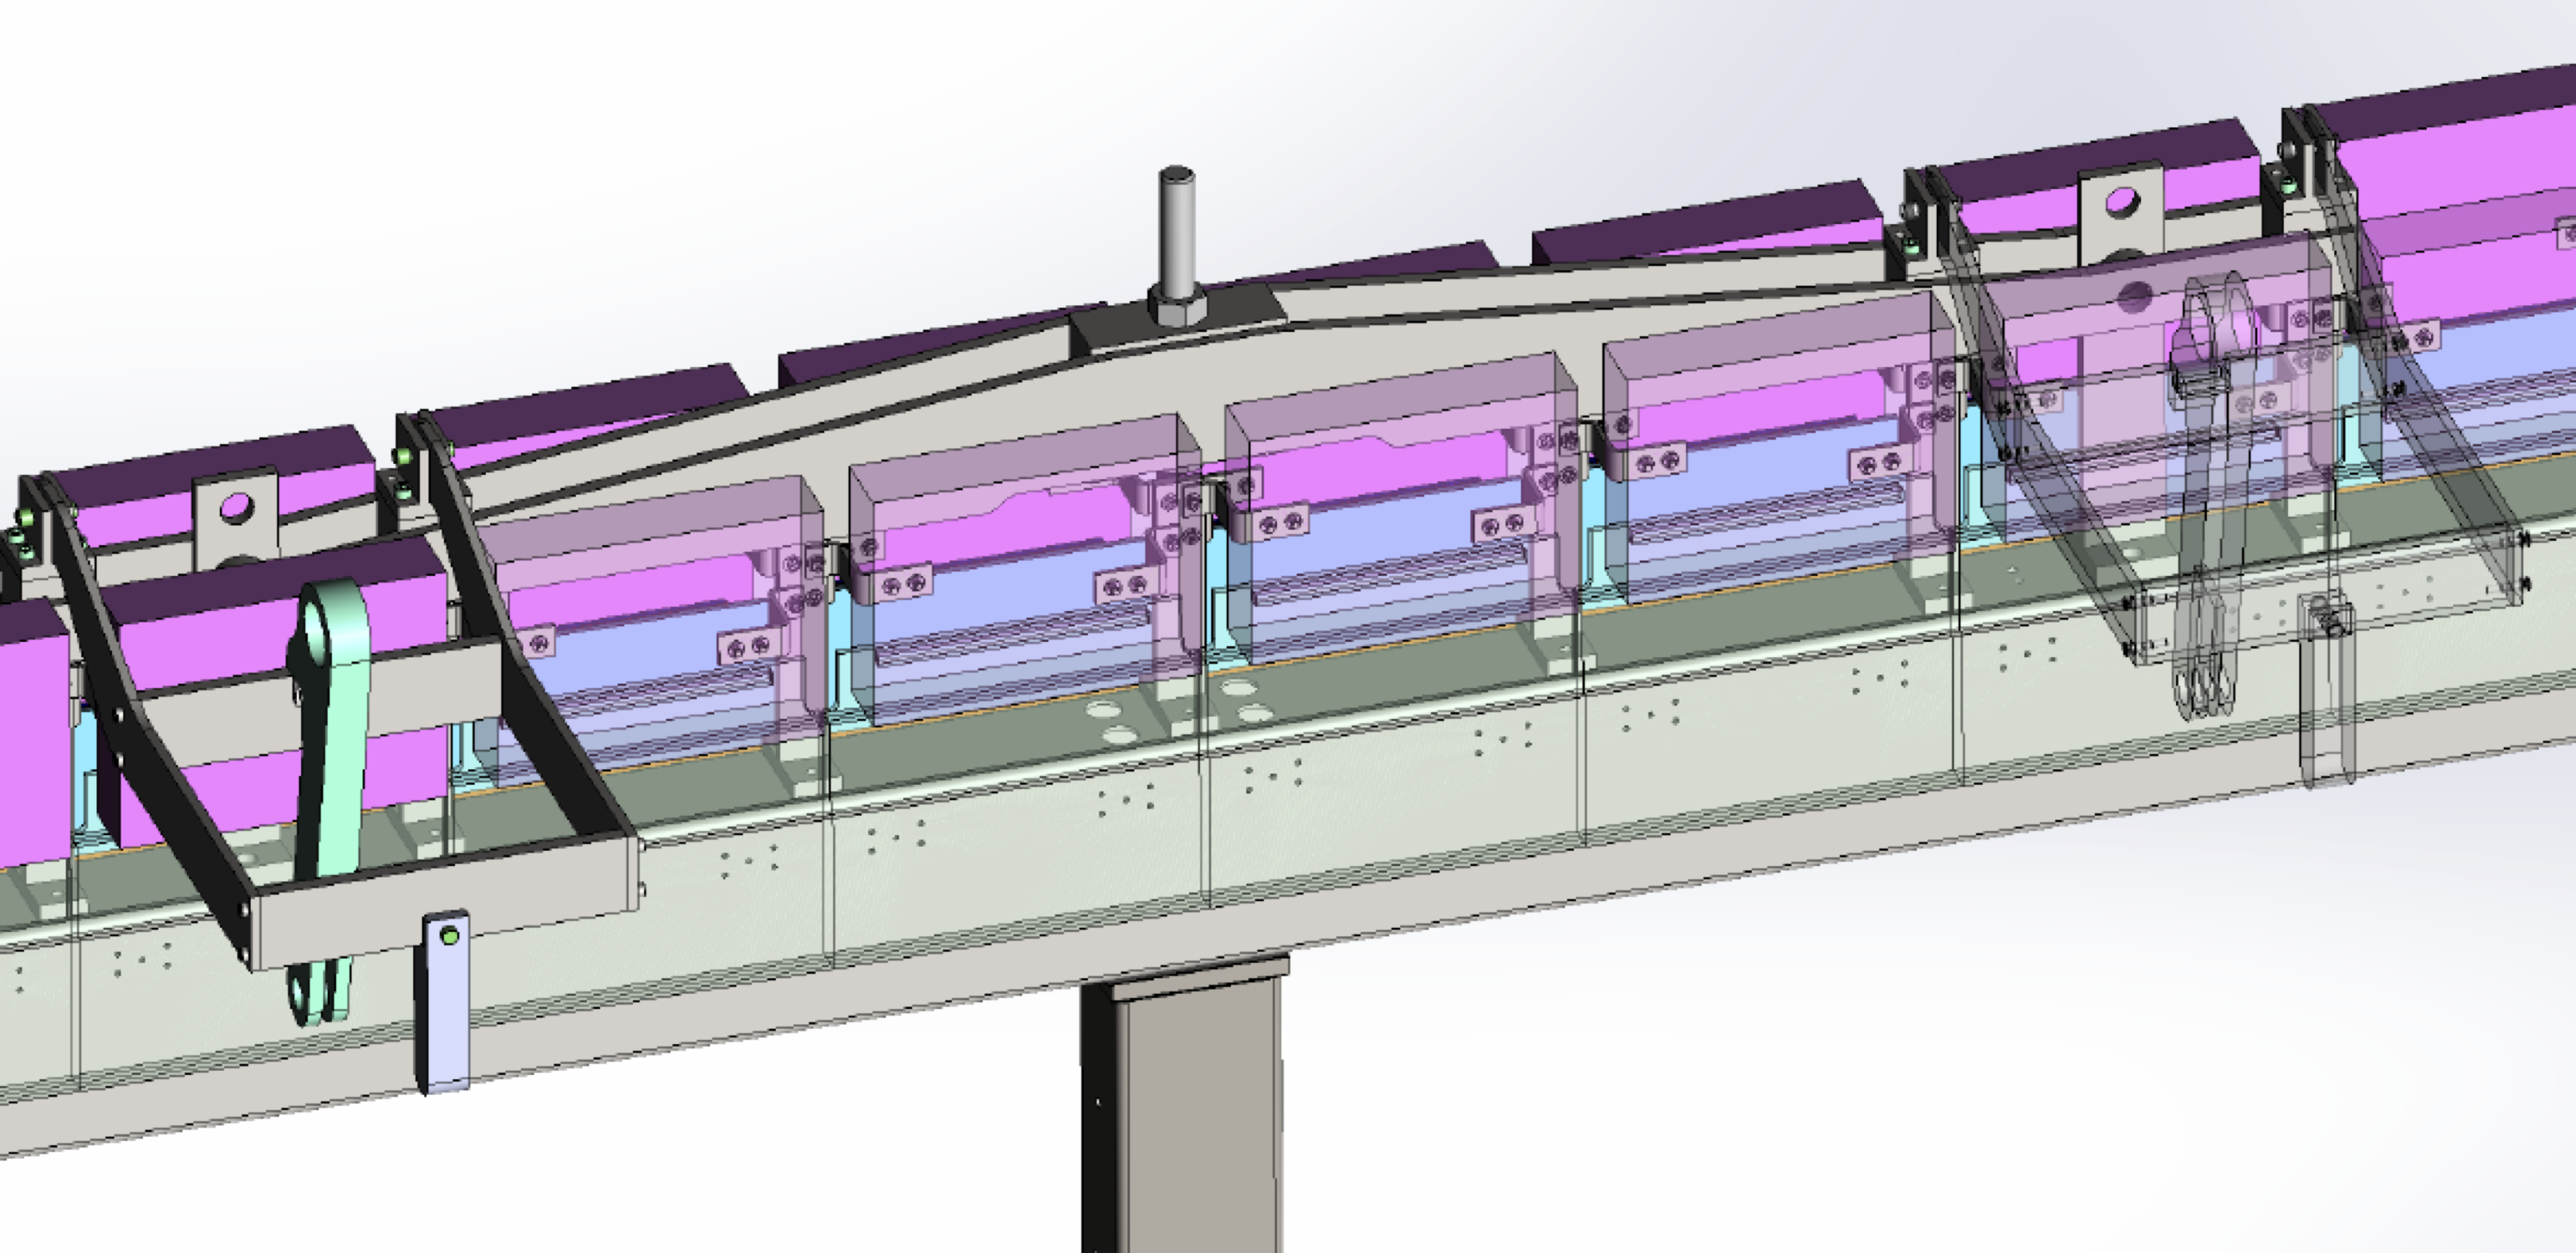
\includegraphics[width=0.9\textwidth]{figures/tpc_apa_electronicsmountingdiagram.png} 
\end{cdrfigure}

%%%%%%%%%%%%
\subsubsection{Comb wire supports on inner frame members}
\label{subsec:apa_combs}

%\paragraph{Purpose}

Some wire segments are long.  The longitudinal wires extend from one end of the APA to the other without going around a side -- a length of 6 m.  Even the diagonal wires across the middle of the APA are 3.9 m long.  To prevent deflection from gravity, electrostatic forces, or liquid drag from moving argon, the wires are supported at regular locations along the length of the APA.  This is done with ``combs'' mounted on each of the four cross braces that are ~ evenly spaced along the length of the APA.  This keeps the longest unsupported wire length under 1.6 m.

The nominal wire tension is 5 N but even the 1.6 m long wires could fall to 3 N of tension before the wire, held horizontally, would deviate 150 microns -- one wire diameter.  In operation the wires are either vertical or 35.7$^{\circ}$ from vertical so the actual deviation would be less.

%\paragraph{Geometry}

The combs are made from 0.5 mm thick G10 with slots cut into it.  The comb for the lowest layer is glued to a base strip that's glued to the frame.  After each layer is wound another comb strip is glued to the tips of the teeth of the previous one to locate the wires in the next layer.  Each successive comb holds the previous layer of wires in the bottom of their slots (Figure \ref{fig:tpc_apa_supportcombmodel}).

\begin{cdrfigure}[APA Support Comb Model]{tpc_apa_supportcombmodel}{A model of the combs showing how they stack.  After winding a layer the comb for the next layer is put in place.  Each comb hold the wires from the previous layer in their slots.}
\includegraphics[width=0.9\textwidth]{figures/tpc_apa_supportcombmodel.png} 
\end{cdrfigure}

Periodic holes along the length of the strip allow the use of pins to accurately locate each successive strip with the previous one.  A series of jigs are used to create and install these combs.  One jig aligns the first strip to the base strip during gluing.  Another jig locates this assembly on the frame as it is glued in place. A third jig locates each successive comb using the previously mentioned registration holes.

The wire openings in the comb stack are small enough that the wires are accurately positioned at the combs.  They are not, however, deliberately glued at the combs.  

%%%%%%%%%%%%
\subsubsection{APA interconnection features}

Some sort of constraint is needed between adjacent APAs to keep them in a plane with each other.  It is also important that this constraint not apply a vertical load to adjacent APAs.  The constraint therefore takes the form of a pair of pins protruding from one edge of the APA (one high and one low on the APA) and a pair of matching slots on the other edge to engage the pins (Figure \ref{fig:tpc_apa_pinslotdrawing}).

\begin{cdrfigure}[APA Interconnect Drawing]{tpc_apa_pinslotdrawing}{The pin/slot constraint.  The pin screws into an insert in the outside frame member of one APA and engages a slot in the outside frame member of the adjacent APA.}
\includegraphics[width=0.9\textwidth]{figures/tpc_apa_pinslotdrawing.png} 
\end{cdrfigure}

Electronic noise concerns have made it desirable to isolate APAs from each other.  To help with that this alignment pin, although it will have a steel core for strength, will have a G10 sleeve where it contacts the frame of the adjacent APA.


 %%%%%%%%%%%%%%%%%%%%%%%%
\subsection{Tests and surveys}

\fixme{Suggest editing this down quite a bit. Anne}

 %%%%%%%%%%%%
 \subsubsection{Tension survey}

Wire tension is a critical parameter in the performance of the APA, and needs to be strictly controlled to ensure the detector will be robust to operation in a cryogenic environment.  As each wireplane layer is added to the APA, and before the next layer is added and restricts access, the tension of every newly added wire will be measured.  Any wire that is more than 1.0 N out of tolerance from the design value of 5.0 N will be removed and, if possible, replaced.  The tension measurement is performed using a laser-photodiode system, developed at PSL and integrated into the wire-winding apparatus, which will record the resonant frequency of a plucked wire.  Visible checks will also be made during production to identify any noticeably sagging wires.  Spot checks of tension will also be made after cryogenic testing at the production site, as well as at CERN prior to insertion of an APA into the protoDUNE cryostat.  

 %%%%%%%%%%%%
\subsubsection{Electrical continuity test}

The electrical connection of each APA wire to the cold readout electronics must be verified to ensure a minimum ($<$0.5$\%$) of un-reachable channels in the completed detector.  Un-reachable wires (e.g. originating from cold solder joints or wires that are broken but held in place by epoxy bead) are distinct from clearly broken wires (e.g. obvious strands of wires hanging loose from the APA) which will be removed/replaced during production.   In addition to providing a pathway to record detector signals, wires receive their bias voltage via their connection to the readout electronics, which shapes the electric field in the anode region.  As such, disconnected wires impact the signals that surrounding channels will collect.  As each wireplane layer is added to the APA, and before the next layer is added and restricts access, the electrical connection of every newly added wire to the corresponding wire-bonding board will be verified.  Using a multimeter, or other equivalent methods, the continuity will be verified by directly probing between the ``bottom" end (i.e. - the end that terminates on the non electronics-plate end of the APA) of the wire and the signal trace on the wire-bonding board at the ``top" end (i.e. - the end that terminates on the electronic-plate end of the APA).  Any wire that fails this continuity test, by producing a resistance $>$ 500 $\Omega$ (using 4.4 $\Omega$/m resistance for BeCu wire that is 7.5 m long, and allowing margin for additional parasitic resistance), will be removed and, if possible, replaced.  Spot checks of continuity will also be made after cryogenic testing at the production site, as well as at CERN prior to insertion of an APA into the protoDUNE cryostat.

 %%%%%%%%%%%%
\subsubsection{Electrical isolation test}

Each wire of the APA should be electrically isolated from every other wire, in order to avoid shorting out channels and potentially damaging the readout electronics.  Shorted-out wires will also impact the electric-field uniformity in the anode region, and can impact signals in surrounding channels.  Using a multimeter, or other equivalent methods, the isolation between each APA wire and adjacent wires will be measured and verified to have resistance $>$ 1 M$\Omega$.  Since a given wire has many adjacent wires, a dedicated circuit designed to expedite this test will be desirable.  Any wire failing this test will be removed and, if possible, replaced.  Visible checks will also be made during production to identify any touching wires.  Spot checks of isolation will also be made after cryogenic testing at the production site, as well as at CERN prior to insertion of an APA into the protoDUNE cryostat.

 %%%%%%%%%%%%
\subsubsection{Wire position survey}

Knowledge of the position of every wire in the APA is required in order for physics analysis of data to be successful.  This information is utilized to create a description of the detector geometry inside the simulation software, and is the basis on which reconstruction algorithms are built. The preliminary description of the geometry assumes a perfect detector built according to the APA design drawings.  Any deviations from this design in the final as-built APAs needs to be incorporated into the software geometry.  All wires should be surveyed during production to verify they are within 500 $\mu$m of the design location.  This survey is partially accomplished by verifying the APA flame flatness is within specifications, and that the wire-bonding boards and support combs are located upon the frame in the desired position.  The APA will be surveyed using a Cognex camera integrated into the winding machine.  The camera employs machine vision to identify each pin/tooth on the installed wire-bonding boards, and from this data a map of wire location will be generated.  This survey should be performed as each wireplane layer is added to the APA, and before the next layer is added and restricts access.  Any wire that is more than 500 $\mu$m from the nominal location, according to survey data, should be inspected and if found to have problems, removed and replaced.  Visual checks throughout the wire-winding process will also be performed to identify any wires that appear out of place.

 %%%%%%%%%%%%
\subsubsection{Bias voltage test}

All wires on the APA must be able to reach their design bias voltage in order to achieve the desired electric-field uniformity and transparency conditions required for successful LArTPC operation.  Inability to reach the desired voltage could be an indication of component failure on the CR boards, or of wires in the APA being shorted out.  The CR boards should be tested prior to their installation on the APA to verify they can be biased to 100$\%$ of the largest operating voltage of any anode layer (e.g. the Collection layer's 820 V).  The components selected for the CR boards are chosen with margin about this operating point, to allow for bias voltages in the as-built detector to be adjusted, either for signal-shaping studies or for systematic studies of detector performance at various drift-field values.  As each wireplane layer is added to the APA, and before the next layer is added and restricts access, each newly added wire-bonding board should be connected to a CR board and biased to 100$\%$ of the largest operating voltage of any anode layer.  Any unexpected current draws observed will be traced to the originating wire(s), and if necessary, the offending wire(s) will be replaced.  Visual checks should also be performed during this test to verify that wires being biased do not deflect or move in any unexpected manner.  This test may be augmented when multiple wireplane layers are available, to verify that wires in adjacent layers do not develop unexpected cross-talk when biased.

 %%%%%%%%%%%%
\subsubsection{Cryogenic test}

The completed APAs must be robust to operation in a cryogenic environment.  Wires must be able to withstand the cooldown to liquid argon temperatures.  In order to verify the workmanship of each APA, a cryogenic test will be performed as each APA is completed and before shipment to CERN.  The APAs will be placed in a custom-built cold box, where they will be gradually cooled (at a rate consistent with requirements on keeping wire tension increases below a safe level) to $\sim$100 K (exact value to be determined).  The default plan is to use cold gas from a LN supply for this test, and flush gas through the cold box until it reaches the desired temperature.  The APA will be arranged in a horizontal orientation, as this simplifies the engineering of the cold box.  It is not anticipated that loading on the APA/wires due to gravity (e.g. from horizontal vs. vertical orientation) will lead to any significant changes in wire tension, and the frame will be supported appropriately.  The APA will be inspected after this cold test to verify that no wires have broken.  Spot-check tests of tension/continuity/isolation/bias will be performed to verify if any channels have changed relative to their pre cold-test values.  Criteria for acceptance after this test (e.g. number of problematic wires identified by this test) are under development.

 %%%%%%%%%%%%
\subsubsection{Testing at CERN}

Upon arrival at CERN, and prior to integration with interfacing subsystems (e.g. - light collection and electronics), each APA will be subjected to visual inspection, and spot-check ($\sim$10$\%$ of total channels) tests for wire tension, continuity, isolation, and bias voltage will be performed and compared to the equivalent pre-shipping values.


